\documentclass[letterpaper]{article} % DO NOT CHANGE THIS
\usepackage{aaai2027} % DO NOT CHANGE THIS
\usepackage[hyphens]{url} % DO NOT CHANGE THIS
\usepackage{graphicx} % DO NOT CHANGE THIS
\urlstyle{rm} % DO NOT CHANGE THIS
\def\UrlFont{\rm} % DO NOT CHANGE THIS
\usepackage{natbib} % DO NOT CHANGE THIS
\usepackage{caption} % DO NOT CHANGE THIS
\frenchspacing % DO NOT CHANGE THIS
\usepackage{amsmath}
\usepackage{amssymb}
\usepackage{booktabs}
\usepackage[brazil]{babel}
\pdfinfo{
/TemplateVersion (2027.1)
}

% Set counter for section numbers (0 means no numbers, 1 means section numbers, 2 means sections and subsections)
\setcounter{secnumdepth}{2}

% Custom commands for diacritics / accented characters
\newcommand{\aacute}{\'a}
\newcommand{\eacute}{\'e}
\newcommand{\iacute}{\'i}
\newcommand{\oacute}{\'o}
\newcommand{\uacute}{\'u}
\newcommand{\acrase}{\`a}
\newcommand{\acirc}{\^a}
\newcommand{\ecirc}{\^e}
\newcommand{\ocirc}{\^o}
\newcommand{\atilde}{\~a}
\newcommand{\otilde}{\~o}
\newcommand{\ccedil}{\c{c}}
\newcommand{\Aacute}{\'A}
\newcommand{\Eacute}{\'E}
\newcommand{\Iacute}{\'I}
\newcommand{\Oacute}{\'O}
\newcommand{\Uacute}{\'U}
\newcommand{\Acrase}{\`A}
\newcommand{\Acirc}{\^A}
\newcommand{\Ecirc}{\^E}
\newcommand{\Ocirc}{\^O}
\newcommand{\Atilde}{\~A}
\newcommand{\Otilde}{\~O}
\newcommand{\Ccedil}{\c{C}}
\newcommand{\cao}{{\ccedil}{\atilde}o}

\renewcommand{\a}{{\acrase}}
\newcommand{\abstracao}{abstra{\cao}}
\newcommand{\aceleracao}{acelera{\cao}}
\newcommand{\acrescimo}{acr{\eacute}scimo}
\newcommand{\Acuracia}{Acur{\aacute}cia}
\newcommand{\acuracia}{acur{\aacute}cia}
\newcommand{\alcancando}{alcan{\ccedil}ando}
\newcommand{\alcancou}{alcan{\c{c}}ou}
\newcommand{\Alem}{Al{\eacute}m}
\newcommand{\alem}{al{\eacute}m}
\newcommand{\alteracao}{altera{\c{c}}{\~a}o}
\newcommand{\alucinacoes}{alucina{\ccedil}{\otilde}es}
\newcommand{\Analise}{An{\aacute}lise}
\newcommand{\analise}{an{\aacute}lise}
\newcommand{\analiticas}{anal{\iacute}ticas}
\newcommand{\analitico}{anal{\iacute}tico}
\newcommand{\ancora}{{\^{a}}ncora}
\newcommand{\AntiTrapaca}{Anti-Trapa{\ccedil}a}
\newcommand{\antitrapaca}{anti-trapa{\ccedil}a}
\newcommand{\aplicacao}{aplica{\cao}}
\newcommand{\apos}{ap{\oacute}s}
\newcommand{\aproximacao}{aproxima{\cao}}
\newcommand{\aquisicao}{aquisi{\cao}}
\newcommand{\arcabouco}{arcabou{\ccedil}o}
\newcommand{\as}{{\acrase}s}
\newcommand{\assintotica}{assint{\oacute}tica}
\newcommand{\ate}{at{\eacute}}
\newcommand{\atribuicao}{atribui{\cao}}
\newcommand{\ausencia}{aus{\^{e}}ncia}
\newcommand{\automatico}{autom{\aacute}tico}
\newcommand{\Avaliacao}{Avalia{\cao}}
\newcommand{\avaliacao}{avalia{\cao}}
\newcommand{\avaliacoes}{avalia{\ccedil}{\otilde}es}
\newcommand{\avancada}{avan{\c{c}}ada}
\newcommand{\avancado}{avan{\ccedil}ado}
\newcommand{\avancados}{avan{\ccedil}ados}
\newcommand{\avanco}{avan{\c{c}}o}
\newcommand{\avancos}{avan{\c{c}}os}
\newcommand{\avancou}{avan{\c{c}}ou}
\newcommand{\balanco}{balan{\ccedil}o}
\newcommand{\basica}{b{\aacute}sica}
\newcommand{\beneficios}{benef{\'{i}}cios}
\newcommand{\binario}{bin{\'{a}}rio}
\newcommand{\caracteristica}{caracter{\iacute}stica}
\newcommand{\carencia}{car{\^{e}}ncia}
\newcommand{\catastrofica}{catastr{\'{o}}fica}
\newcommand{\cenarios}{cen{\aacute}rios}
\newcommand{\centralizacao}{centraliza{\cao}}
\newcommand{\cientifica}{cient{\iacute}fica}
\newcommand{\classificacao}{classifica{\cao}}
\newcommand{\Classificacao}{Classifica{\cao}}
\newcommand{\Codigo}{C{\oacute}digo}
\newcommand{\codigo}{c{\oacute}digo}
\newcommand{\codigos}{c{\oacute}digos}
\newcommand{\coerencia}{coer{\ecirc}ncia}
\newcommand{\combinacao}{combina{\c{c}}{\~a}o}
\newcommand{\comparacao}{compara{\cao}}
\newcommand{\compativeis}{compat{\iacute}veis}
\newcommand{\composicao}{composi{\cao}}
\newcommand{\concluida}{conclu{\iacute}da}
\newcommand{\Conclusao}{Conclus{\atilde}o}
\newcommand{\conclusao}{conclus{\~a}o}
\newcommand{\conclusoes}{conclus{\~o}es}
\newcommand{\Conclusoes}{Conclus{\~o}es}
\newcommand{\condicoes}{condi{\ccedil}{\otilde}es}
\newcommand{\confianca}{confian{\ccedil}a}
\newcommand{\constroi}{constr{\oacute}i}
\newcommand{\contem}{cont{\eacute}m}
\newcommand{\contencao}{conten{\cao}}
\newcommand{\Contingencia}{Conting{\ecirc}ncia}
\newcommand{\contingencia}{conting{\ecirc}ncia}
\newcommand{\continuo}{cont{\iacute}nuo}
\newcommand{\contrario}{contr{\aacute}rio}
\newcommand{\Convergencia}{Converg{\ecirc}ncia}
\newcommand{\convergencia}{converg{\ecirc}ncia}
\newcommand{\correcao}{corre{\cao}}
\newcommand{\Criterio}{Crit{\eacute}rio}
\newcommand{\criterio}{crit{\eacute}rio}

\newcommand{\declaracao}{declara{\cao}}
\newcommand{\decompoe}{decomp{\otilde}e}
\newcommand{\Decomposicao}{Decomposi{\cao}}
\newcommand{\decomposicao}{decomposi{\cao}}
\newcommand{\decorrencia}{decorr{\ecirc}ncia}
\newcommand{\deducao}{dedu{\cao}}
\newcommand{\definicao}{defini{\cao}}
\newcommand{\delimitacao}{delimita{\cao}}
\newcommand{\demonstracao}{demonstra{\cao}}
\newcommand{\demonstracoes}{demonstra{\ccedil}{\otilde}es}
\newcommand{\dependencias}{depend{\^{e}}ncias}
\newcommand{\descalibracoes}{descalibra{\c{c}}{\~o}es}
\newcommand{\descricao}{descri{\cao}}
\newcommand{\deteccao}{detec{\cao}}
\newcommand{\deterministico}{determin{\iacute}stico}
\newcommand{\deterministicos}{determin{\'{i}}sticos}
\newcommand{\dialogo}{di{\aacute}logo}
\newcommand{\diaria}{di{\aacute}ria}
\newcommand{\diarias}{di{\aacute}rias}
\newcommand{\Diferenca}{Diferen{\ccedil}a}
\newcommand{\diferenca}{diferen{\ccedil}a}
\newcommand{\diferencas}{diferen{\ccedil}as}
\newcommand{\dinamica}{din{\acirc}mica}
\newcommand{\dinamicas}{din{\acirc}micas}
\newcommand{\Dinamica}{Din{\acirc}mica}
\newcommand{\direcao}{dire{\c{c}}{\~a}o}
\newcommand{\discrepancia}{discrep{\^{a}}ncia}
\newcommand{\discrepancias}{discrep{\^{a}}ncias}
\newcommand{\Discussao}{Discuss{\atilde}o}
\newcommand{\discussao}{discuss{\~a}o}
\newcommand{\dispendio}{disp{\ecirc}ndio}
\newcommand{\disponibilizacao}{disponibiliza{\cao}}
\newcommand{\distribuicao}{distribui{\cao}}
\newcommand{\Distribuicao}{Distribui{\cao}}
\newcommand{\distribuicoes}{distribui{\ccedil}{\otilde}es}
\newcommand{\distribuidos}{distribu{\'{i}}dos}
\newcommand{\divergencia}{diverg{\ecirc}ncia}
\newcommand{\divergencias}{diverg{\ecirc}ncias}
\newcommand{\dominio}{dom{\iacute}nio}
\newcommand{\e}{{\eacute}}
\newcommand{\eficacia}{efic{\aacute}cia}
\newcommand{\Eficacia}{Efic{\aacute}cia}
\newcommand{\eficiencia}{efici{\ecirc}ncia}
\newcommand{\elevacao}{eleva{\cao}}
\newcommand{\Elicitacao}{Elicita{\cao}}
\newcommand{\elicitacao}{elicita{\cao}}
\newcommand{\emissao}{emiss{\atilde}o}
\newcommand{\empirica}{emp{\iacute}rica}
\newcommand{\Empirico}{Emp{\iacute}rico}
\newcommand{\empirico}{emp{\iacute}rico}
\newcommand{\empiricos}{emp{\iacute}ricos}
\newcommand{\entao}{ent{\~a}o}
\newcommand{\equilibrio}{equil{\iacute}brio}
\newcommand{\equivalencia}{equival{\ecirc}ncia}
\newcommand{\escalavel}{escal{\'{a}}vel}
\newcommand{\esforco}{esfor{\ccedil}o}
\newcommand{\espaco}{espa{\ccedil}o}
\newcommand{\espacos}{espa{\c{c}}os}
\newcommand{\especificacao}{especifica{\cao}}
\newcommand{\especificas}{espec{\iacute}ficas}
\newcommand{\espuria}{esp{\'{u}}ria}
\newcommand{\espurias}{esp{\uacute}rias}
\newcommand{\Espurio}{Esp{\uacute}rio}
\newcommand{\espurio}{esp{\uacute}rio}
\newcommand{\Estatistica}{Estat{\iacute}stica}
\newcommand{\estatistica}{estat{\iacute}stica}
\newcommand{\estatistico}{estat{\iacute}stico}
\newcommand{\estatisticos}{estat{\iacute}sticos}
\newcommand{\estavel}{est{\'{a}}vel}
\newcommand{\estimacao}{estima{\cao}}
\newcommand{\estimulo}{est{\'{i}}mulo}
\newcommand{\estocastica}{estoc{\aacute}stica}
\newcommand{\estocasticas}{estoc{\'{a}}sticas}
\newcommand{\estocastico}{estoc{\aacute}stico}
\newcommand{\estrategia}{estrat{\'{e}}gia}
\newcommand{\estrategias}{estrat{\eacute}gias}
\newcommand{\evolucao}{evolu{\cao}}
\newcommand{\Execucao}{Execu{\cao}}
\newcommand{\execucao}{execu{\cao}}
\newcommand{\execucoes}{execu{\ccedil}{\otilde}es}
\newcommand{\executaveis}{execut{\'{a}}veis}
\newcommand{\executavel}{execut{\aacute}vel}
\newcommand{\existencia}{exist{\^{e}}ncia}
\newcommand{\explicita}{expl{\iacute}cita}
\newcommand{\explicitacao}{explicita{\cao}}
\newcommand{\explicitas}{expl{\iacute}citas}
\newcommand{\expoe}{exp{\otilde}e}
\newcommand{\expressao}{express{\~a}o}
\newcommand{\extensoes}{extens{\otilde}es}
\newcommand{\familias}{fam{\iacute}lias}
\newcommand{\fenomeno}{fen{\ocirc}meno}
\newcommand{\fenomenos}{fen{\ocirc}menos}
\newcommand{\finalizacao}{finaliza{\cao}}
\newcommand{\flutuacoes}{flutua{\c{c}}{\~o}es}
\newcommand{\forca}{for{\ccedil}a}
\newcommand{\forcar}{for{\ccedil}ar}
\newcommand{\Formulacao}{Formula{\cao}}
\newcommand{\formulacao}{formula{\cao}}
\newcommand{\frequencia}{frequ{\ecirc}ncia}
\newcommand{\funcao}{fun{\cao}}
\newcommand{\funcoes}{fun{\ccedil}{\otilde}es}
\newcommand{\Fundamentacao}{Fundamenta{\cao}}
\newcommand{\fundamentacao}{fundamenta{\cao}}
\newcommand{\generalizacao}{generaliza{\cao}}
\newcommand{\geometrica}{geom{\'{e}}trica}
\newcommand{\geometricas}{geom{\eacute}tricas}
\newcommand{\geometricosemantica}{geom{\eacute}trico-sem{\acirc}ntica}
\newcommand{\geracao}{gera{\cao}}
\newcommand{\Gestao}{Gest{\atilde}o}
\newcommand{\gestao}{gest{\atilde}o}
\newcommand{\hegemonico}{hegem{\^{o}}nico}
\newcommand{\hermetico}{herm{\'{e}}tico}
\newcommand{\heuristicos}{heur{\'{i}}sticos}
\newcommand{\Hipotese}{Hip{\oacute}tese}
\newcommand{\hipotese}{hip{\oacute}tese}
\newcommand{\Hipoteses}{Hip{\oacute}teses}
\newcommand{\hipoteses}{hip{\oacute}teses}
\newcommand{\identicas}{id{\ecirc}nticas}
\newcommand{\impar}{{\'{i}}mpar}
\newcommand{\impoe}{imp{\otilde}e}
\newcommand{\importacao}{importa{\cao}}
\newcommand{\importacoes}{importa{\ccedil}{\otilde}es}
\newcommand{\incidencia}{incid{\^{e}}ncia}
\newcommand{\incongruencias}{incongru{\^{e}}ncias}
\newcommand{\incorrecoes}{incorre{\ccedil}{\otilde}es}
\newcommand{\indexacao}{indexa{\c{c}}{\~a}o}
\newcommand{\Indice}{{\Iacute}ndice}
\newcommand{\indice}{{\iacute}ndice}
\newcommand{\indices}{{\iacute}ndices}
\newcommand{\indispensavel}{indispens{\'{a}}vel}
\newcommand{\ineditas}{in{\'{e}}ditas}
\newcommand{\Inferencia}{Infer{\ecirc}ncia}
\newcommand{\inferencia}{infer{\ecirc}ncia}
\newcommand{\insercao}{inser{\cao}}
\newcommand{\instrucoes}{instru{\ccedil}{\otilde}es}
\newcommand{\instruidos}{instru{\iacute}dos}
\newcommand{\integracao}{integra{\cao}}
\newcommand{\inteligencia}{intelig{\ecirc}ncia}
\newcommand{\interacao}{intera{\c{c}}{\~a}o}
\newcommand{\Intermediaria}{Intermedi{\'{a}}ria}
\newcommand{\intermediarias}{intermedi{\'{a}}rias}
\newcommand{\intermediario}{intermedi{\'{a}}rio}
\newcommand{\intermediarios}{intermedi{\aacute}rios}
\newcommand{\interrupcoes}{interrup{\ccedil}{\otilde}es}
\newcommand{\Introducao}{Introdu{\cao}}
\newcommand{\introducao}{introdu{\cao}}
\newcommand{\intuia}{intu{\'{i}}a}
\newcommand{\invariancia}{invari{\acirc}ncia}
\newcommand{\inversao}{invers{\~a}o}
\newcommand{\investigacao}{investiga{\c{c}}{\~a}o}
\newcommand{\iteracao}{itera{\cao}}
\newcommand{\iteracoes}{itera{\ccedil}{\otilde}es}
\newcommand{\Iteracao}{Itera{\cao}}
\newcommand{\ja}{j{\aacute}}
\newcommand{\Ja}{J{\'{a}}}
\newcommand{\Latencia}{Lat{\^{e}}ncia}
\newcommand{\latencia}{lat{\^{e}}ncia}
\newcommand{\logica}{l{\oacute}gica}
\newcommand{\logicogeometricas}{l{\'{o}}gico-geom{\'{e}}tricas}
\newcommand{\mandatoria}{mandat{\'{a}}ria}
\newcommand{\mandatorias}{mandat{\'{a}}rias}
\newcommand{\mandatorio}{mandat{\oacute}rio}
\newcommand{\maximo}{m{\aacute}ximo}
\newcommand{\medias}{m{\'{e}}dias}
\newcommand{\medio}{m{\eacute}dio}
\newcommand{\memorizacao}{memoriza{\cao}}
\newcommand{\mensuracao}{mensura{\cao}}
\newcommand{\metodo}{m{\eacute}todo}
\newcommand{\metodologica}{metodol{\oacute}gica}
\newcommand{\metodologico}{metodol{\oacute}gico}
\newcommand{\metodos}{m{\eacute}todos}
\newcommand{\metricas}{m{\eacute}tricas}
\newcommand{\microscopica}{microsc{\'{o}}pica}
\newcommand{\minimo}{m{\iacute}nimo}
\newcommand{\modulos}{m{\oacute}dulos}
\newcommand{\multiplas}{m{\uacute}ltiplas}
\newcommand{\nao}{n{\atilde}o}
\newcommand{\Nao}{N{\atilde}o}
\newcommand{\naoparametrica}{n{\~a}o-param{\'{e}}trica}
\newcommand{\naoparametrico}{n{\atilde}o-param{\eacute}trico}
\newcommand{\naoparametricos}{n{\atilde}o-param{\eacute}tricos}
\newcommand{\naosuperioridade}{n{\~a}o-superioridade}
\newcommand{\necessaria}{necess{\aacute}ria}
\newcommand{\necessario}{necess{\aacute}rio}
\newcommand{\niveis}{n{\'{i}}veis}
\newcommand{\nivel}{n{\iacute}vel}
\newcommand{\notavel}{not{\aacute}vel}
\newcommand{\numero}{n{\uacute}mero}
\newcommand{\observacoes}{observa{\ccedil}{\otilde}es}
\newcommand{\Obtencao}{Obten{\cao}}
\newcommand{\obtencao}{obten{\cao}}
\newcommand{\ocorrencia}{ocorr{\ecirc}ncia}
\newcommand{\operacoes}{opera{\ccedil}{\otilde}es}
\newcommand{\orcamento}{or{\c{c}}amento}
\newcommand{\oscilacoes}{oscila{\ccedil}{\otilde}es}
\newcommand{\otica}{{\'{o}}tica}
\newcommand{\padrao}{padr{\atilde}o}
\newcommand{\padroes}{padr{\otilde}es}
\newcommand{\padronizacao}{padroniza{\c{c}}{\~a}o}
\newcommand{\parametros}{par{\acirc}metros}
\newcommand{\passiveis}{pass{\iacute}veis}
\newcommand{\permutacao}{permuta{\cao}}
\newcommand{\Permutacao}{Permuta{\cao}}
\newcommand{\Persistencia}{Persist{\ecirc}ncia}
\newcommand{\porem}{por{\eacute}m}
\newcommand{\possivel}{poss{\iacute}vel}
\newcommand{\pratica}{pr{\'{a}}tica}
\newcommand{\presenca}{presen{\ccedil}a}
\newcommand{\previa}{pr{\'{e}}via}
\newcommand{\previas}{pr{\'{e}}vias}
\newcommand{\previo}{pr{\'{e}}vio}
\newcommand{\primario}{prim{\'{a}}rio}
\newcommand{\programacao}{programa{\cao}}
\newcommand{\Proibicao}{Proibi{\cao}}
\newcommand{\propensao}{propens{\~a}o}
\newcommand{\propoe}{prop{\otilde}e}
\newcommand{\proprietarios}{propriet{\aacute}rios}
\newcommand{\quantificacao}{quantifica{\c{c}}{\~a}o}
\newcommand{\raciocinio}{racioc{\iacute}nio}
\newcommand{\ramificacoes}{ramifica{\ccedil}{\otilde}es}
\newcommand{\realimentacao}{realimenta{\cao}}
\newcommand{\recemapresentado}{rec{\'{e}}m-apresentado}
\newcommand{\Recuperacao}{Recupera{\cao}}
\newcommand{\recuperacao}{recupera{\cao}}
\newcommand{\recuperacoes}{recupera{\ccedil}{\otilde}es}
\newcommand{\reducao}{redu{\cao}}
\newcommand{\referencia}{refer{\ecirc}ncia}
\newcommand{\reflexao}{reflex{\~a}o}
\newcommand{\Regressao}{Regress{\atilde}o}
\newcommand{\regressao}{regress{\atilde}o}
\newcommand{\regressoes}{regress{\otilde}es}
\newcommand{\relacao}{rela{\cao}}
\newcommand{\relevancia}{relev{\^{a}}ncia}
\newcommand{\repertorio}{repert{\oacute}rio}
\newcommand{\replicas}{r{\eacute}plicas}
\newcommand{\reposicao}{reposi{\cao}}
\newcommand{\Repositorio}{Reposit{\oacute}rio}
\newcommand{\Representacao}{Representa{\cao}}
\newcommand{\representacao}{representa{\cao}}
\newcommand{\reprodutiveis}{reprodut{\iacute}veis}
\newcommand{\reprodutivel}{reprodut{\'{i}}vel}
\newcommand{\reproduzivel}{reproduz{\iacute}vel}
\newcommand{\requisicao}{requisi{\cao}}
\newcommand{\requisicoes}{requisi{\ccedil}{\otilde}es}
\newcommand{\resiliencia}{resili{\ecirc}ncia}
\newcommand{\resolucao}{resolu{\cao}}
\newcommand{\restricao}{restri{\cao}}
\newcommand{\restricoes}{restri{\ccedil}{\otilde}es}
\newcommand{\Restricoes}{Restri{\ccedil}{\otilde}es}
\newcommand{\retroalimentacao}{retroalimenta{\c{c}}{\~a}o}
\newcommand{\rigidas}{r{\iacute}gidas}
\newcommand{\rigido}{r{\iacute}gido}
\newcommand{\ruido}{ru{\iacute}do}
\newcommand{\saida}{sa{\'{i}}da}
\newcommand{\saidas}{sa{\iacute}das}
\newcommand{\sao}{s{\atilde}o}
\newcommand{\saturacao}{satura{\cao}}
\newcommand{\Secao}{Se{\cao}}
\newcommand{\secao}{se{\c{c}}{\~a}o}
\newcommand{\secoes}{se{\c{c}}{\~o}es}
\newcommand{\Secoes}{Se{\c{c}}{\~o}es}
\newcommand{\selecao}{sele{\c{c}}{\~a}o}
\newcommand{\Semantica}{Sem{\acirc}ntica}
\newcommand{\semantica}{sem{\acirc}ntica}
\newcommand{\semanticas}{sem{\acirc}nticas}
\newcommand{\Semantico}{Sem{\acirc}ntico}
\newcommand{\semantico}{sem{\acirc}ntico}
\newcommand{\semanticos}{sem{\acirc}nticos}
\newcommand{\sensivel}{sens{\iacute}vel}
\newcommand{\significancia}{signific{\acirc}ncia}
\newcommand{\simbolica}{simb{\'{o}}lica}
\newcommand{\simultanea}{simult{\acirc}nea}
\newcommand{\simultaneo}{simult{\^{a}}neo}
\newcommand{\sintatica}{sint{\'{a}}tica}
\newcommand{\sintaticas}{sint{\aacute}ticas}
\newcommand{\Sintese}{S{\iacute}ntese}
\newcommand{\sintese}{s{\iacute}ntese}
\newcommand{\sintetico}{sint{\eacute}tico}
\newcommand{\sistematicas}{sistem{\aacute}ticas}
\newcommand{\situacao}{situa{\cao}}
\newcommand{\solucao}{solu{\cao}}
\newcommand{\solucoes}{solu{\ccedil}{\otilde}es}
\newcommand{\tambem}{tamb{\eacute}m}
\newcommand{\teoricoestatistica}{te{\oacute}rico-estat{\iacute}stica}
\newcommand{\tolerancia}{toler{\acirc}ncia}
\newcommand{\transformacao}{transforma{\cao}}
\newcommand{\transformacoes}{transforma{\c{c}}{\~o}es}
\newcommand{\Transicoes}{Transi{\ccedil}{\otilde}es}
\newcommand{\transicoes}{transi{\ccedil}{\otilde}es}
\newcommand{\translacao}{transla{\cao}}
\newcommand{\tres}{tr{\^{e}}s}
\newcommand{\Tres}{Tr{\^{e}}s}
\newcommand{\unica}{{\uacute}nica}
\newcommand{\unico}{{\'{u}}nico}
\newcommand{\util}{{\'{u}}til}
\newcommand{\validacao}{valida{\cao}}
\newcommand{\Validacao}{Valida{\cao}}
\newcommand{\validas}{v{\'{a}}lidas}
\newcommand{\valido}{v{\'{a}}lido}
\newcommand{\variacao}{varia{\cao}}
\newcommand{\Variacoes}{Varia{\ccedil}{\otilde}es}
\newcommand{\variacoes}{varia{\ccedil}{\otilde}es}
\newcommand{\variavel}{vari{\aacute}vel}
\newcommand{\vazao}{vaz{\atilde}o}
\newcommand{\verificacao}{verifica{\cao}}
\newcommand{\visiveis}{vis{\iacute}veis}
\newcommand{\visivel}{vis{\iacute}vel}

\newcommand{\Ameaca}{Amea\c{c}a}
\newcommand{\Apos}{Ap\'{o}s}
\newcommand{\Especificacao}{Especifica\c{c}\~{a}o}
\newcommand{\Geometricas}{Geom\'{e}tricas}
\newcommand{\Hermetico}{Herm\'{e}tico}
\newcommand{\Imposicao}{Imposi\c{c}\~{a}o}
\newcommand{\Limitacoes}{Limita\c{c}\~{o}es}
\newcommand{\Minima}{M\'{i}nima}
\newcommand{\Neurosimbolica}{Neurosimb\'{o}lica}
\newcommand{\Orcamento}{Or\c{c}amento}
\newcommand{\Parametros}{Par\^{a}metros}
\newcommand{\Psicometrica}{Psicom\'{e}trica}
\newcommand{\Seguranca}{Seguran\c{c}a}
\newcommand{\absorcao}{absor\c{c}\~{a}o}
\newcommand{\adocao}{ado\c{c}\~{a}o}
\newcommand{\alcancar}{alcan\c{c}ar}
\newcommand{\aleatorias}{aleat\'{o}rias}
\newcommand{\aleatorios}{aleat\'{o}rios}
\newcommand{\algoritmica}{algor\'{i}tmica}
\newcommand{\algoritmico}{algor\'{i}tmico}
\newcommand{\analises}{an\'{a}lises}
\newcommand{\atencao}{aten\c{c}\~{a}o}
\newcommand{\avancar}{avan\c{c}ar}
\newcommand{\basico}{b\'{a}sico}
\newcommand{\cirurgicos}{cir\'{u}rgicos}
\newcommand{\clausulas}{cl\'{a}usulas}
\newcommand{\coloracao}{colora\c{c}\~{a}o}
\newcommand{\comparacoes}{compara\c{c}\~{o}es}
\newcommand{\competencia}{compet\^{e}ncia}
\newcommand{\concentracao}{concentra\c{c}\~{a}o}
\newcommand{\concordancia}{concord\^{a}ncia}
\newcommand{\consonancia}{conson\^{a}ncia}
\newcommand{\contornaveis}{contorn\'{a}veis}
\newcommand{\convergencias}{converg\^{e}ncias}
\newcommand{\criacao}{cria\c{c}\~{a}o}
\newcommand{\criterios}{crit\'{e}rios}
\newcommand{\celulas}{c\'{e}lulas}
\newcommand{\dependencia}{depend\^{e}ncia}
\newcommand{\destruicao}{destrui\c{c}\~{a}o}
\newcommand{\deterministica}{determin\'{i}stica}
\newcommand{\dimensao}{dimens\~{a}o}
\newcommand{\direcoes}{dire\c{c}\~{o}es}
\newcommand{\discordancia}{discord\^{a}ncia}
\newcommand{\digitos}{d\'{i}gitos}
\newcommand{\empiricas}{emp\'{i}ricas}
\newcommand{\especificacoes}{especifica\c{c}\~{o}es}
\newcommand{\especificos}{espec{\iacute}ficos}
\newcommand{\espurios}{esp\'{u}rios}
\newcommand{\estagnacao}{estagna\c{c}\~{a}o}
\newcommand{\estatica}{est\'{a}tica}
\newcommand{\estaticos}{est\'{a}ticos}
\newcommand{\evidencia}{evid\^{e}ncia}
\newcommand{\exatidao}{exatid\~{a}o}
\newcommand{\excecao}{exce\c{c}\~{a}o}
\newcommand{\exigencia}{exig\^{e}ncia}
\newcommand{\exploracao}{explora\c{c}\~{a}o}
\newcommand{\expressoes}{express\~{o}es}
\newcommand{\flexivel}{flex\'{i}vel}
\newcommand{\generalizavel}{generaliz\'{a}vel}
\newcommand{\geometricos}{geom\'{e}tricos}
\newcommand{\historico}{hist\'{o}rico}
\newcommand{\implicacoes}{implica\c{c}\~{o}es}
\newcommand{\inclusao}{inclus\~{a}o}
\newcommand{\inducao}{indu\c{c}\~{a}o}
\newcommand{\inicializacao}{inicializa\c{c}\~{a}o}
\newcommand{\instrucao}{instru\c{c}\~{a}o}
\newcommand{\interdicao}{interdi\c{c}\~{a}o}
\newcommand{\intermediaria}{intermedi\'{a}ria}
\newcommand{\interpretacao}{interpreta\c{c}\~{a}o}
\newcommand{\interpretacoes}{interpreta\c{c}\~{o}es}
\newcommand{\intrinseca}{intr\'{i}nseca}
\newcommand{\intrinsecas}{intr\'{i}nsecas}
\newcommand{\inversoes}{invers\~{o}es}
\newcommand{\lexicografica}{lexicogr\'{a}fica}
\newcommand{\logicos}{l\'{o}gicos}
\newcommand{\memorizacoes}{memoriza\c{c}\~{o}es}
\newcommand{\metodologicos}{metodol\'{o}gicos}
\newcommand{\monocromatico}{monocrom\'{a}tico}
\newcommand{\morfologica}{morfol\'{o}gica}
\newcommand{\media}{m\'{e}dia}
\newcommand{\minimos}{m\'{i}nimos}
\newcommand{\negligencia}{neglig\^{e}ncia}
\newcommand{\neurosimbolicos}{neurosimb\'{o}licos}
\newcommand{\obtem}{obt\'{e}m}
\newcommand{\ocorrencias}{ocorr\^{e}ncias}
\newcommand{\oferecam}{ofere\c{c}am}
\newcommand{\ordenacao}{ordena\c{c}\~{a}o}
\newcommand{\organizacao}{organiza\c{c}\~{a}o}
\newcommand{\orientacao}{orienta\c{c}\~{a}o}
\newcommand{\poligono}{pol\'{i}gono}
\newcommand{\preteritas}{pret\'{e}ritas}
\newcommand{\primaria}{prim\'{a}ria}
\newcommand{\prioritarias}{priorit\'{a}rias}
\newcommand{\probabilistico}{probabil\'{i}stico}
\newcommand{\programatica}{program\'{a}tica}
\newcommand{\proporcoes}{propor\c{c}\~{o}es}
\newcommand{\provavel}{prov\'{a}vel}
\newcommand{\psicometrica}{psicom\'{e}trica}
\newcommand{\publica}{p\'{u}blica}
\newcommand{\questao}{quest\~{a}o}
\newcommand{\reforcando}{refor\c{c}ando}
\newcommand{\rejeicao}{rejei\c{c}\~{a}o}
\newcommand{\replicacao}{replica\c{c}\~{a}o}
\newcommand{\retem}{ret\'{e}m}
\newcommand{\revisao}{revis\~{a}o}
\newcommand{\rigidos}{r\'{i}gidos}
\newcommand{\sintatico}{sint\'{a}tico}
\newcommand{\submissao}{submiss\~{a}o}
\newcommand{\subordinacao}{subordina\c{c}\~{a}o}
\newcommand{\teorica}{te\'{o}rica}
\newcommand{\teoricas}{te\'{o}ricas}
\newcommand{\termico}{t\'{e}rmico}
\newcommand{\verbalizacao}{verbaliza\c{c}\~{a}o}
\newcommand{\valida}{v\'{a}lida}
\newcommand{\Arvore}{\'{A}rvore}
\newcommand{\Arvores}{\'{A}rvores}
\newcommand{\Unica}{\'{U}nica}
\newcommand{\ambito}{\^{a}mbito}
\newcommand{\multiplos}{m{\'{u}}ltiplos}
\newcommand{\vitorias}{vit{\'{o}}rias}


\renewcommand{\tablename}{Tabela}
\renewcommand{\figurename}{Figura}
\renewcommand{\refname}{Refer{\^e}ncias}

\title{\Analise{} do Impacto de \Variacoes{} de Prompting e Feedback \Semantico{} no ARC-AGI-1: \Fundamentacao{} \Estatistica{}}

\author{
    Fabio Luiz da Costa Cieslak\equalcontrib\textsuperscript{1},
    Izadora Candotti de Oliveira\equalcontrib\textsuperscript{1},
    Matheus Machado\equalcontrib\textsuperscript{1}
}
\affiliations{
    Universidade Federal do Rio Grande do Sul\textsuperscript{1}
}

\begin{document}

\maketitle

\begin{abstract}
O benchmark \textit{Abstraction and Reasoning Corpus} (ARC-AGI-1) avalia o \raciocinio{} indutivo e a \generalizacao{} em sistemas de \inteligencia{} artificial por meio da \transformacao{} de grades matriciais coloridas a partir de \demonstracoes{} visuais. Neste trabalho investiga-se a \sintese{} indutiva de programas guiada por contraexemplos (CEGIS) e o efeito de \restricoes{} textuais \AntiTrapaca{} sobre oito modelos de linguagem em 100 tarefas do benchmark. A variante \AntiTrapaca{}, que restringe desvios condicionais ad-hoc e demanda a \declaracao{} \previa{} do invariante abstrato, revelou-se estatisticamente equivalente ao CEGIS \padrao{} ($50{,}4\%$ vs.\ $49{,}8\%$, $p = 0{,}5515$), refutando a \hipotese{} de que diretivas de prompt anti-hardcoding oferecem vantagem \generalizavel{}. A \analise{} dos modos de falha revelou que, embora o teto de busca responda por $86{,}9\%$ dos erros no agregado, o sobreajuste \espurio{} \e{} a barreira dominante na fronteira ($100\%$ no \texttt{Grok 4.6} e $71{,}4\%$ no \texttt{DeepSeek V4}).
\end{abstract}

\section{\Introducao{}}
O \textit{Abstraction and Reasoning Corpus} (ARC-AGI) \cite{chollet2019measure} foi proposto para mensurar a \inteligencia{} geral por meio da \inducao{}, contrastando com a \memorizacao{} em bases massivas \caracteristica{} dos Grandes Modelos de Linguagem (LLMs). Cada tarefa \e{} composta por matrizes bidimensionais discretas com valores inteiros de 0 a 9 (representando dez cores distintas), acompanhadas de 2 a 5 pares de treino (entrada e \saida{} esperada) e uma grade de teste oculta, cuja \transformacao{} deve ser inferida com \exatidao{}.

Neste trabalho, explora-se a \sintese{} indutiva de programas guiada por contraexemplos (CEGIS, \textit{Counterexample-Guided Inductive Synthesis}) \cite{solar2008program} para resolver tarefas ARC-AGI usando LLMs. A \inducao{} de programas a partir de demonstra{\c{c}}{\~o}es matriciais alinha-se a marcos do dom{\'{i}}nio, como o aprendizado de invariantes e linguagens conceituais no DreamCoder \cite{ellis2021dreamcoder} e a comunica{\c{c}}{\~a}o de programas naturais no corpus LARC \cite{larc2022acquaviva}. Em contraste com \metodos{} dedutivos cl{\'{a}}ssicos baseados em provadores \logicos{} e \especificacoes{} completas, o CEGIS sintetiza \funcoes{} em Python sob supervis{\~a}o de exemplos \empiricos{}. O LLM atua como sintetizador \probabilistico{}, enquanto o interpretador atua como verificador \deterministico{}. Essa din{\^{a}}mica conecta-se aos paradigmas de auto-reparo e \reflexao{} verbal em LLMs, como \textit{Self-Refine} \cite{madaan2023self} e \textit{Reflexion} \cite{shinn2023reflexion}, nos quais a cadeia de \raciocinio{} \cite{wei2022chain} \e{} direcionada pela \evidencia{} do erro.

Devido \a{} estrutura do CEGIS, \e{} \possivel{} que ocorram \solucoes{} parciais para as tarefas, nas quais o modelo adiciona condicionais ou dados \especificos{} das tarefas de treino (hardcoded) que \nao{} generalizam para as tarefas de teste. Para investigar esse \fenomeno{}, \propoe{}-se um teste entre dois prompts de contraexemplo: um com diretivas denominadas \AntiTrapaca{} e outro sem. O objetivo dessas regras \e{} coibir \memorizacoes{} parciais por meio do veto a regras ad-hoc e da \exigencia{} de \verbalizacao{} do invariante subjacente. A \hipotese{} central deste trabalho \e{} que \textit{\restricoes{} \semanticas{} anti-hardcoding e a \reflexao{} \explicita{} sobre invariantes melhoram a taxa de acerto no teste oculto do ARC-AGI}. Para isso, estabelece-se um protocolo experimental pareado no benchmark, avaliando formalmente oito modelos de linguagem em uma amostra controlada de 100 tarefas.

\section{\Sintese{} de Programas e \Variacoes{} de Prompting}
\label{sec:metodo}

\subsection{Ciclo Conversacional do CEGIS \Semantico{}}
Diferentemente de avalia{\c{c}}{\~o}es baseadas em amostragem paralela (\textit{pass@k} com m{\'{u}}ltiplas gera{\c{c}}{\~o}es independentes), neste trabalho o \textit{pass@1} designa estritamente o Turno 0 de uma sess{\~a}o conversacional interativa \textit{stateful} com or{\c{c}}amento de reparos $K_{\max} = 5$. No Turno 0, o modelo recebe as \demonstracoes{} de treino e sintetiza a \funcao{} candidata \texttt{transform(grid)}. Para isolar o \codigo{} \executavel{} do texto explicativo, o sistema utiliza \expressoes{} regulares para extrair exclusivamente o bloco delimitado por \texttt{\`{}\`{}\`{}python ... \`{}\`{}\`{}}, prevenindo falhas de \interpretacao{} decorrentes de prosa adicional.

A din{\^{a}}mica iterativa obedece a tr{\^{e}}s pol{\'{i}}ticas formais: (i)~\textbf{Parada Estrita (\textit{Hard Stopping}):} em cada turno $k \in \{0, \dots, K_{\max}-1\}$, a fun{\c{c}}{\~a}o candidata \e{} executada sequencialmente sobre os pares de treino. Obtendo 100\% de conformidade no treino, o ciclo de busca \e{} encerrado imediatamente e o c{\'{o}}digo \e{} submetido {\`{a}} grade de teste oculta. Logo, solu{\c{c}}{\~o}es que acertam o treino no Turno 0 (\textit{pass@1}) s{\~a}o preservadas sem altera{\c{c}}{\~o}es, impossibilitando regress{\~a}o no treino; (ii)~\textbf{Interrup{\c{c}}{\~a}o no Primeiro Contraexemplo:} havendo erro de sintaxe, \textit{timeout} de $2{,}0\text{s}$ ou diverg{\^{e}}ncia matricial, a execu{\c{c}}{\~a}o interrompe no primeiro exemplo discordante, gerando feedback corretivo; e (iii)~\textbf{Esgotamento de Or{\c{c}}amento:} atingindo $K_{\max} = 5$ itera{\c{c}}{\~o}es sem converg{\^{e}}ncia no treino, a sess{\~a}o encerra-se como falha e o teste cego n{\~a}o \e{} consultado.

\subsection{Diretivas \AntiTrapaca{} e \Elicitacao{} de Invariantes}
Modelos submetidos a feedback de contraexemplos podem cair em sobreajuste (\textit{overfitting}), inserindo \clausulas{} condicionais dedicadas unicamente a satisfazer o exemplo discordante rec{\'{e}}m-apresentado. A \estrategia{} \AntiTrapaca{} estabelece \instrucoes{} negativas expressas contra \ramificacoes{} ad-hoc e exige que o modelo explicite o conceito invariante antes de redigir o \codigo{}.

Ressalta-se que a \restricao{} \a{} coordenadas fixas e a \exigencia{} do invariante foram aplicadas exclusivamente via engenharia de prompt conversacional, sem filtragem ou \rejeicao{} \programatica{} em tempo de \execucao{} no sandbox. Como ferramenta auditora \textit{post-hoc}, utilizou-se uma varredura baseada em \expressoes{} regulares sobre as 2.398 \funcoes{} geradas, inspecionando \padroes{} de coordenadas e matrizes literais.

\subsection{\Especificacao{} Estruturada dos Prompts}
Para assegurar a estrita replicabilidade do estudo, o protocolo estabeleceu o texto literal dos blocos de \instrucao{}:

\noindent\textbf{1. Prompt de Sistema:} \textit{"You are an expert AI solving ARC-AGI puzzles by writing Python code."}

\noindent\textbf{2. Prompt Inicial de Passada \Unica{} (pass@1):}
Apresenta os pares de treino serializados em JSON (\texttt{Example 0}, etc.), requisita a \funcao{} \texttt{transform(grid)} e estipula o bloco \texttt{ANTI\_IMPORT}:
\begin{quote}\footnotesize\ttfamily\raggedright\setlength{\topsep}{1.5pt}\setlength{\partopsep}{0pt}
CODE RULES:\\
- DO NOT use any `import` statements (e.g., collections, numpy, math, etc.).\\
- USE ONLY pure native Python types and functions (list, dict, set, tuple, range, len, min, max, sum, enumerate, zip, abs).
\end{quote}

\noindent\textbf{3. Feedback de Contraexemplo (CEGIS):}
As grades 2D s{\~a}o serializadas em matrizes JSON (\texttt{json.dumps()}, e.g., \texttt{[[0,1],[2,3]]}). Sob falha no treino $i$, o sistema emite o feedback literal:
\begin{quote}\footnotesize\ttfamily\raggedright\setlength{\topsep}{1.5pt}\setlength{\partopsep}{0pt}
Your code failed on Training Example \{i\}.\\
- Input: <json\_input\_grid>\\
- Expected Output: <json\_expected\_grid>\\
- Produced Output:\\
  <json\_produced\_grid | Execution Error: ...>\\ \relax
[CODE RULES ...]\\
Analyze the discrepancy, fix your logic, and provide the updated `transform(grid)` function inside a ```python ... ``` block.
\end{quote}

\noindent\textbf{4. Diretivas Adicionais (\AntiTrapaca{}):}
Anexa textualmente ao feedback de contraexemplo o bloco literal \texttt{ANTI\_CHEAT}:
\begin{quote}\footnotesize\ttfamily\raggedright\setlength{\topsep}{1.5pt}\setlength{\partopsep}{0pt}
- DO NOT add conditional branches (if/else) targeting specific example indices, hardcoded coordinates, or specific row values of a single training case. The transformation must be a single, uniform mathematical/geometric rule that applies to ALL grids identically.\\
- Before writing the code, explicitly state the single abstract invariant that explains why the previous code failed on Example X and how the new logic naturally handles Examples 0, 1, and 2 without special cases.
\end{quote}

\section{Metodologia e \Fundamentacao{} \Estatistica{}}
\label{sec:estatistica}
\subsection{\Analise{} Pareada, Permuta{\c{c}}{\~a}o e Bootstrap}
Para comparar o desempenho das estratégias mantendo a estrutura pareada, utilizamos um teste de permutação com 100.000 réplicas. O teste exato de McNemar foi aplicado aos pares discordantes, e a reamostragem bootstrap pareada (10.000 réplicas) determinou os intervalos de confiança de 95\%. O controle da taxa de erro familiar para os 8 modelos avaliados foi feito com a correção de Bonferroni ($\alpha = 0,00625$).

\subsection{\Classificacao{} dos Modos de Falha}
As falhas na \sintese{} \sao{} categorizados em:
(i)~\textbf{Sobreajuste \Espurio{} (Falsa \Convergencia{}):} o \codigo{} \obtem{} sucesso em $100\%$ das \demonstracoes{} de treino, \porem{} falha na grade de teste cego devido \a{} \absorcao{} de regras acidentais; e
(ii)~\textbf{Teto de Busca e \Representacao{}:} o processo \nao{} converge no conjunto de treino dentro das $K_{\max} = 5$ \iteracoes{} concedidas.

% Auto-generated combined summary table
\begin{table*}[t]
  \centering
  \small
  \caption{Resultados consolidados nos 100 problemas avaliados do ARC-AGI-1 sob os regimes de tentativa única (pass@1), CEGIS e CEGIS com \AntiTrapaca{} ($N=100$). Acurácias expressas em percentual; as colunas de tarefas recuperadas e requisições médias por problema qualificam o processo iterativo do CEGIS Semântico.}
  \label{tab:combined_results}
  \begin{tabular}{l c cccc cc}
    \toprule
    & \multicolumn{1}{c}{Baseline} & \multicolumn{4}{c}{CEGIS Sem\^antico} & \multicolumn{2}{c}{CEGIS + \AntiTrapaca{}} \\
    \cmidrule(lr){2-2} \cmidrule(lr){3-6} \cmidrule(lr){7-8}
    Modelo & Acur\'acia (\%) & Acur\'acia (\%) & $\Delta$ (pp) & Recuperadas & Req./Tarefa & Acur\'acia (\%) & $\Delta$ (pp) \\
    \midrule
    \texttt{Grok 4.6} & 88 & 92 & +4 & 4 & 1.13 & 92 & +0 \\
    \texttt{DeepSeek V4 Flash 0731} & 74 & 86 & +12 & 12 & 1.25 & 86 & +0 \\
    \texttt{GPT-5.6 Luna} & 58 & 77 & +19 & 19 & 2.00 & 79 & +2 \\
    \texttt{Claude Sonnet 5} & 32 & 62 & +30 & 30 & 2.90 & 60 & -2 \\
    \texttt{Gemini 3.5 Flash Lite} & 21 & 43 & +22 & 22 & 3.23 & 45 & +2 \\
    \texttt{Gemini 3.1 Flash Lite} & 12 & 31 & +19 & 19 & 4.07 & 24 & -7 \\
    \texttt{Leanstral 1.5.1} & 3 & 7 & +4 & 4 & 4.69 & 9 & +2 \\
    \texttt{GPT-5.4 Nano} & 1 & 5 & +4 & 4 & 4.89 & 3 & -2 \\
    \bottomrule
  \end{tabular}
\end{table*}

% Auto-generated statistical significance and error taxonomy table
\begin{table*}[t]
  \centering
  \small
  \caption{Testes de \significancia{} \estatistica{} pareada (\permutacao{} e Bootstrap, $B=10{.}000$) e \decomposicao{} de erros sob feedback \semantico{} ($\alpha = 0{,}05$).}
  \label{tab:significance_tests}
  \setlength{\tabcolsep}{4.5pt}
  \begin{tabular}{lcccccc}
    \toprule
    Modelo & $\Delta_{\text{CEGIS}}$ & $p_{\text{perm}}$ (CEGIS) & $p_{\text{boot}}$ (CEGIS) & IC 95\% Bootstrap & Sobreajuste \Espurio{} & Teto Repres. \\
    \midrule
    \texttt{Grok 4.6} & +4.0\% & 0.0603 & 0.0431 & [1.0\%, 8.0\%] & 8 & 0 \\
    \texttt{DeepSeek V4 Flash 0731} & +12.0\% & 0.0005 & 0.0007 & [6.0\%, 19.0\%] & 10 & 4 \\
    \texttt{GPT-5.6 Luna} & +19.0\% & 0.0001 & 0.0001 & [12.0\%, 27.0\%] & 10 & 13 \\
    \texttt{Claude Sonnet 5} & +30.0\% & 0.0001 & 0.0001 & [21.0\%, 39.0\%] & 7 & 31 \\
    \texttt{Gemini 3.5 Flash Lite} & +22.0\% & 0.0001 & 0.0001 & [14.0\%, 30.0\%] & 10 & 47 \\
    \texttt{Gemini 3.1 Flash Lite} & +19.0\% & 0.0001 & 0.0001 & [12.0\%, 27.0\%] & 7 & 62 \\
    \texttt{Leanstral 1.5.1} & +4.0\% & 0.0603 & 0.0457 & [1.0\%, 8.0\%] & 0 & 93 \\
    \texttt{GPT-5.4 Nano} & +4.0\% & 0.0603 & 0.0496 & [1.0\%, 8.0\%] & 0 & 95 \\
    \bottomrule
  \end{tabular}
\end{table*}


\section{Protocolo Experimental e \Execucao{}}
\label{sec:experimento}

\subsection{Sandbox e \Seguranca{} de \Execucao{}}
O \codigo{} sintetizado \e{} executado em subprocesso isolado via \texttt{multiprocessing} com \inicializacao{} estrita em contexto \textit{spawn} e limite de tempo de $2{,}0\text{s}$. Interceptores nativos do interpretador (\texttt{sys.addaudithook}) bloqueiam chamadas de disco (\texttt{open}), conectores de rede (\texttt{socket}), \criacao{} de processos (\texttt{subprocess}) e \importacoes{} (\texttt{import}). A \execucao{} \e{} restrita a uma lista de tipos e \funcoes{} (\texttt{\_SAFE\_BUILTINS}). O \criterio{} de \validacao{} \e{} exato e estrito: as matrizes de \saida{} geradas devem coincidir com a \referencia{} em \dimensao{} e \coloracao{}.

\subsection{Modelos, Amostragem e \Parametros{} de \Inferencia{}}
Avaliou-se um painel com oito modelos: de fronteira (\texttt{Grok 4.6}, \texttt{DeepSeek V4 Flash 0731} e \texttt{GPT-5.6 Luna}), intermedi{\'{a}}rios (\texttt{Claude Sonnet 5}, \texttt{Gemini 3.5 Flash Lite} e \texttt{Gemini 3.1 Flash Lite}) e compactos (\texttt{Leanstral 1.5.1} e \texttt{GPT-5.4 Nano}). A amostragem compreendeu 100 tarefas de treino do ARC-AGI-1 selecionadas pela ordena{\c{c}}{\~a}o lexicogr{\'{a}}fica dos identificadores hexadecimais (\texttt{00576224} a \texttt{3aa6fb7a}) gerados na cria{\c{c}}{\~a}o do corpus \cite{chollet2019measure}. A infer{\^{e}}ncia empregou temperatura $T = 0{,}2$, \texttt{top\_p} $= 1{,}0$, limite m{\'{a}}ximo de 4.096 tokens de gera{\c{c}}{\~a}o e sementes determin{\'{i}}sticas nos provedores suportados.

\section{Resultados Experimentais e \Analise{}}
\label{sec:resultados}

O protocolo produziu 800 \execucoes{} pareadas (100 tarefas $\times$ 8 modelos). A Tabela~\ref{tab:combined_results} sintetiza a \acuracia{} global e o custo operacional por modelo, enquanto que a Tabela~\ref{tab:significance_tests} detalha os testes inferenciais e os modos de falha.

\subsection{\Eficacia{} do CEGIS sobre a Passada \Unica{}}
\label{sec:cegis_eficacia}
A Tabela~\ref{tab:significance_tests} confirma que o CEGIS supera significativamente o baseline de passada \unica{} (\textit{pass@1}) em todos os oito modelos avaliados ($+14{,}3$~pp no agregado, $p_{\text{boot}} < 0{,}05$, com intervalos bootstrap estritamente positivos). Sob a pol{\'{i}}tica de parada estrita, solu{\c{c}}{\~o}es bem-sucedidas no treino no Turno 0 s{\~a}o preservadas sem altera{\c{c}}{\~a}o, recuperando 114 tarefas previamente n{\~a}o resolvidas e validando a efic{\'{a}}cia emp{\'{i}}rica do refinamento iterativo.

\subsection{\Decomposicao{} dos Modos de Falha}
\label{sec:modos_falha}
A classifica{\c{c}}{\~a}o das 397 falhas revela que, embora o teto de busca e representa{\c{c}}{\~a}o responda por $86{,}9\%$ dos erros no agregado (345 casos), o sobreajuste esp{\'{u}}rio constitui a barreira prim{\'{a}}ria nos modelos de fronteira, respondendo por $100\%$ das falhas no \texttt{Grok 4.6} (8 erros) e $71{,}4\%$ no \texttt{DeepSeek V4} (10 erros). Em contrapartida, redes compactas falham exclusivamente pela n{\~a}o converg{\^{e}}ncia no treino (95 erros no \texttt{GPT-5.4 Nano} e 93 no \texttt{Leanstral 1.5.1}).

A auditoria estrutural do c{\'{o}}digo revelou ainda uma disparidade sistem{\'{a}}tica no comprimento dos programas segundo o desfecho: fun{\c{c}}{\~o}es associadas a sobreajuste esp{\'{u}}rio apresentaram em m{\'{e}}dia $55{,}9$ linhas de c{\'{o}}digo (SLOC), contra $34{,}6$ linhas nas solu{\c{c}}{\~o}es corretas de primeira tentativa. Esse aumento reflete o ac{\'{u}}mulo de remendos heur{\'{i}}sticos e ramifica{\c{c}}{\~o}es condicionais adicionais ao longo das itera{\c{c}}{\~o}es.

\subsection{CEGIS vs.\ \AntiTrapaca{}: Teste da \Hipotese{} Central}
\label{sec:anticheat_teste}
A Tabela~\ref{tab:anticheat_significance} confronta diretamente o CEGIS \padrao{} com a variante \AntiTrapaca{}. No agregado, a \acuracia{} foi de $50{,}4\%$ contra $49{,}8\%$ (\diferenca{} de $-0{,}6$~pp). A matriz de \contingencia{} pareada contabilizou 45 casos discordantes: $b = 25$ tarefas resolvidas exclusivamente pelo CEGIS e $c = 20$ resolvidas com exclusividade pelo \AntiTrapaca{}. O teste binomial exato de McNemar resultou em $p = 0{,}5515$, enquanto que o intervalo bootstrap \contem{} o zero ($IC_{95\%} [-2{,}25\%, +1{,}00\%]$). 

\Apos{} o controle de Bonferroni para \multiplas{} \comparacoes{} ($\alpha/8 = 0{,}00625$), nenhum modelo isolado atingiu \significancia{} (o menor valor, registrado no \texttt{Gemini 3.1 Flash Lite} com $p_{\text{exact}} = 0{,}0156$, ajusta-se para $p_{\text{bonf}} = 0{,}1250$). Portanto, refuta-se a \hipotese{} de que \instrucoes{} textuais anti-hardcoding \oferecam{} vantagem \generalizavel{}. A Figura~\ref{fig:strategy_discrepancy} resume essa \equivalencia{} estrutural.

\begin{figure}[t]
  \centering
  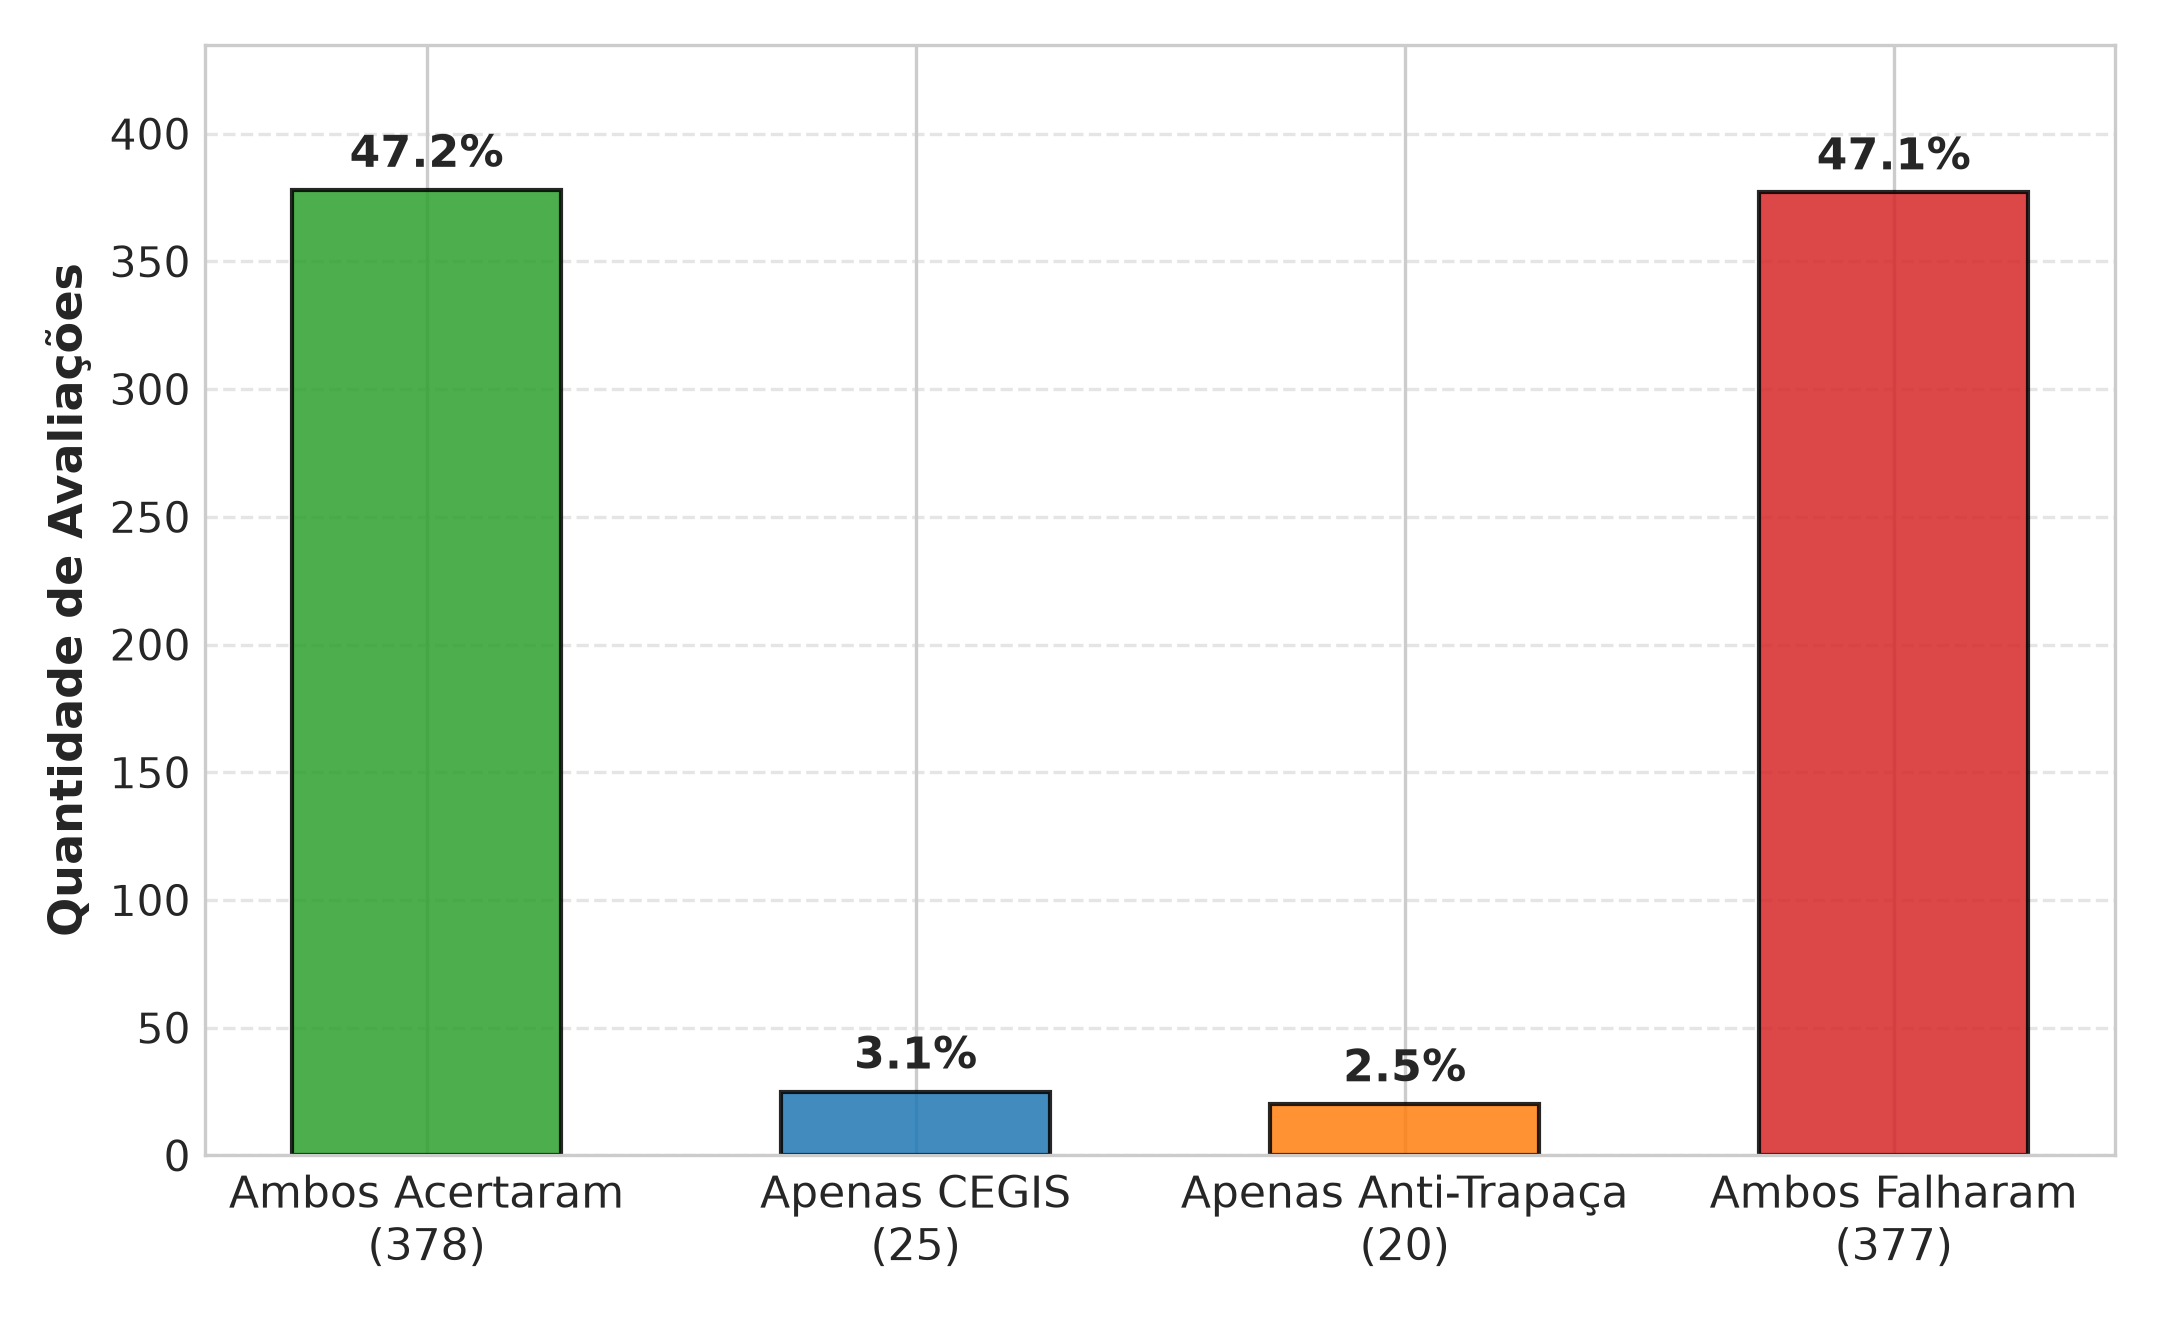
\includegraphics[width=0.92\columnwidth]{static_analysis_output/plot_strategy_discrepancy.png}
  \caption{Distribui{\c{c}}{\~a}o das \execucoes pareados entre CEGIS e \AntiTrapaca{} evidenciando a paridade de desempenho entre os modelos.}
  \label{fig:strategy_discrepancy}
\end{figure}

% Auto-generated statistical significance table: CEGIS vs. AntiCheat
\begin{table*}[t]
  \centering
  \small
  \caption{Testes de \significancia{} pareada para \AntiTrapaca{} vs.\ CEGIS (Binomial Exato, \Permutacao{} e Bootstrap $B=10{,}000$, $\alpha=0{,}05$). Coluna $b / c$: pares discordantes ($b$: exclusivas do CEGIS; $c$: exclusivas do \AntiTrapaca{}).}
  \label{tab:anticheat_significance}
  \setlength{\tabcolsep}{4.5pt}
  \begin{tabular}{lcccccccc}
    \toprule
    Modelo & CEGIS & \AntiTrapaca{} & $\Delta$ & $b / c$ & $p_{\text{exact}}$ & $p_{\text{perm}}$ & IC 95\% Bootstrap & $p_{\text{bonf}}$ \\
    \midrule
    \texttt{Claude Sonnet 5} & 62.0\% & 60.0\% & -2.0\% & 5 / 3 & 0.7266 & 0.7236 & [-8.0\%, +3.0\%] & 1.0000 \\
    \texttt{DeepSeek V4 Flash 0731} & 86.0\% & 86.0\% & +0.0\% & 0 / 0 & 1.0000 & 1.0000 & [+0.0\%, +0.0\%] & 1.0000 \\
    \texttt{GPT-5.4 Nano} & 5.0\% & 3.0\% & -2.0\% & 3 / 1 & 0.6250 & 0.6243 & [-6.0\%, +2.0\%] & 1.0000 \\
    \texttt{GPT-5.6 Luna} & 77.0\% & 79.0\% & +2.0\% & 2 / 4 & 0.6875 & 0.6875 & [-2.0\%, +7.0\%] & 1.0000 \\
    \texttt{Gemini 3.1 Flash Lite} & 31.0\% & 24.0\% & -7.0\% & 7 / 0 & 0.0156 & 0.0178 & [-12.0\%, -3.0\%] & 0.1250 \\
    \texttt{Gemini 3.5 Flash Lite} & 43.0\% & 45.0\% & +2.0\% & 6 / 8 & 0.7905 & 0.7919 & [-5.0\%, +9.0\%] & 1.0000 \\
    \texttt{Grok 4.6} & 92.0\% & 92.0\% & +0.0\% & 0 / 0 & 1.0000 & 1.0000 & [+0.0\%, +0.0\%] & 1.0000 \\
    \texttt{Leanstral 1.5.1} & 7.0\% & 9.0\% & +2.0\% & 2 / 4 & 0.6875 & 0.6861 & [-2.0\%, +7.0\%] & 1.0000 \\
    \midrule
    \textbf{TOTAL AGREGADO} & 50.4\% & 49.8\% & -0.6\% & 25 / 20 & 0.5515 & 0.5501 & [-2.2\%, +1.0\%] & — \\
    \bottomrule
  \end{tabular}
\end{table*}

\section{\Discussao{}}
\label{sec:discussao}
A \avaliacao{} experimental conduz a tr{\^e}s \implicacoes{} \teoricas{} e \empiricas{}:

\noindent\textbf{1. Paridade do \AntiTrapaca{} e Aus{\^e}ncia de Patologia no Baseline:}
A equival{\^{e}}ncia estat{\'{i}}stica observada entre o CEGIS padr{\~a}o e a variante \AntiTrapaca{} decorre de um diagn{\'o}stico emp{\'{i}}rico revelador: os modelos raramente fraudam as demonstra{\c{c}}{\~o}es de treino por meio de coordenadas cartesianas fixas. A auditoria realizada por express{\~o}es regulares sobre as 2.398 fun{\c{c}}{\~o}es geradas identificou apenas 7 ocorr{\^{e}}ncias ($0{,}29\%$) de coordenadas ad-hoc. Contudo, essa taxa afere estritamente a indexa{\c{c}}{\~a}o literal de coordenadas (e.g., \texttt{if r == 3 and c == 5}). Contrastando esse baixo percentual com o incha{\c{c}}o estrutural identificado na Se{\c{c}}{\~a}o~\ref{sec:resultados} ($55{,}9$ vs.\ $34{,}6$ SLOC), constata-se que os modelos sobreajustam por meio de remendos heur{\'{i}}sticos distribu{\'{i}}dos, la{\c{c}}os e condicionais fragmentadas que acomodam os pares de treino sem capturar o invariante global, e n{\~a}o por checagens pontuais de coordenadas. Assim, a restri{\c{c}}{\~a}o a coordenadas literais atacou uma patologia marginal, deixando o sobreajuste heur{\'{i}}stico desregulado. Al{\'{e}}m disso, sem barreiras sint{\'{a}}ticas formais no sandbox, diretivas puramente textuais permanecem vulner{\'{a}}veis {\`{a}} neglig{\^e}ncia instrucional sob racioc{\'{i}}nio complexo.

\noindent\textbf{2. Esgotamento do Or{\c{c}}amento de Busca vs.\ Teto de Representa{\c{c}}{\~a}o:}
Embora o teto de busca e representa{\c{c}}{\~a}o responda por $86{,}9\%$ dos erros no agregado, o sobreajuste esp{\'{u}}rio constitui o obst{\'{a}}culo preponderante na fronteira ($100\%$ no \texttt{Grok 4.6} e $71{,}4\%$ no \texttt{DeepSeek V4}). Para os modelos limitados pelo teto de busca, a n{\~a}o converg{\^{e}}ncia no treino n{\~a}o reflete necessariamente incapacidade representacional inerente. O protocolo operou sob amostragem quase determin{\'{i}}stica ($T=0{,}2$), busca estritamente linear (sem retrocesso) e or{\c{c}}amento restrito de $K_{\max}=5$ turnos, aprisionando o sintetizador em m{\'{i}}nimos locais ap{\'{o}}s o primeiro contraexemplo. Essa limita{\c{c}}{\~a}o aponta que as falhas podem ser causadas pela estrat{\'{e}}gia de explora{\c{c}}{\~a}o e or{\c{c}}amento de busca, super{\'{a}}veis por busca em {\'{a}}rvore (\textit{Tree Search}) ou amostragem paralela, e n{\~a}o unicamente da capacidade intr{\'{i}}nseca das redes.

\noindent\textbf{3. Amea{\c{c}}a {\`{a}} Validade Externa e Contamina{\c{c}}{\~a}o Pr{\'{e}}via:}
Uma salvaguarda metodol{\'{o}}gica cr{\'{i}}tica diz respeito {\`{a}} validade externa dos resultados. Como o corpus p{\'{u}}blico do ARC-AGI-1 foi disponibilizado em 2019, {\'{e}} plaus{\'{i}}vel que modelos de fronteira tenham sido expostos ao conjunto de treino e a reposit{\'{o}}rios comunit{\'{a}}rios durante o pr{\'{e}}-treinamento. Embora o protocolo de CEGIS avalie a capacidade de induzir c{\'{o}}digo sob contraexemplos em tempo de execu{\c{c}}{\~a}o, n{\~a}o se pode descartar que a alta acur{\'{a}}cia inicial reflita memoriza{\c{c}}{\~a}o pr{\'{e}}via de primitivas visuais.

\section{\Limitacoes{} e Trabalhos Futuros}
\label{sec:limitacoes}
As descobertas reportadas delineiam quatro \direcoes{} \prioritarias{}:
(i)~\textbf{Escala de Amostragem:} estender o estudo \as{} 800 tarefas completas do ARC-AGI-1 e ao ARC-AGI-2;
(ii)~\textbf{\Imposicao{}:} substituir diretivas puramente textuais por filtros \estaticos{} \rigidos{} via AST que barrem \ramificacoes{} ad-hoc antes do sandbox;
(iii)~\textbf{Busca em \Arvore{}:} transcender a busca linear \basica{} mediante \textit{Monte Carlo Tree Search} (MCTS) ou amostragem \textit{Best-of-$N$} com escalonamento \termico{} ($\Delta T > 0$); e
(iv)~\textbf{DSLs \Geometricas{}:} atenuar o teto de \representacao{} suprindo primitivas de simetria e conectividade \morfologica{} em vez de Python puro.

\section{\Conclusao{}}
\label{sec:conclusao}
Este trabalho estabeleceu uma investiga{\c{c}}{\~a}o estat{\'{i}}stica acerca da s{\'{i}}ntese indutiva de programas guiada por contraexemplos no ARC-AGI-1, confrontando o protocolo cl{\'{a}}ssico de auto-reparo conversacional com diretivas textuais restritivas anti-hardcoding. A evid{\^{e}}ncia emp{\'{i}}rica coletada sobre oito modelos de linguagem refutou a hip{\'{o}}tese de que as diretivas de prompt negativas utilizadas promovam maior generaliza{\c{c}}{\~a}o para grades ocultas, demonstrando equival{\^{e}}ncia estat{\'{i}}stica entre as abordagens.

A an{\'{a}}lise dos programas sintetizados revelou que essa paridade decorre do vi{\'{e}}s algor{\'{i}}tmico intr{\'{i}}nseco dos grandes modelos de linguagem, que raramente recorrem a ramifica{\c{c}}{\~o}es ad-hoc por coordenadas no baseline ($0{,}29\%$), tornando a restri{\c{c}}{\~a}o textual pontual ineficaz frente ao verdadeiro mecanismo de sobreajuste esp{\'{u}}rio: a infla{\c{c}}{\~a}o estrutural de c{\'{o}}digo por ac{\'{u}}mulo de remendos.

Por fim, a taxonomia de erros evidenciou que a quase totalidade das falhas origina-se da n{\~a}o converg{\^{e}}ncia sobre as demonstra{\c{c}}{\~o}es de treino, e n{\~a}o de sobreajustes esp{\'{u}}rios. Esse achado demonstra que a fronteira de avan{\c{c}}o no ARC-AGI n{\~a}o depende primariamente de ajustes sutis de prompt ou penaliza{\c{c}}{\~o}es de heur{\'{i}}sticas, mas da amplia{\c{c}}{\~a}o do or{\c{c}}amento computacional em tempo de infer{\^{e}}ncia via busca estruturada em {\'{a}}rvore e do suporte a linguagens espec{\'{i}}ficas de dom{\'{i}}nio.

\bibliography{references}

\end{document}